\documentclass[tikz]{standalone}

\usetikzlibrary{automata, positioning, arrows, calc}
\usepackage{relsize}

\begin{document}

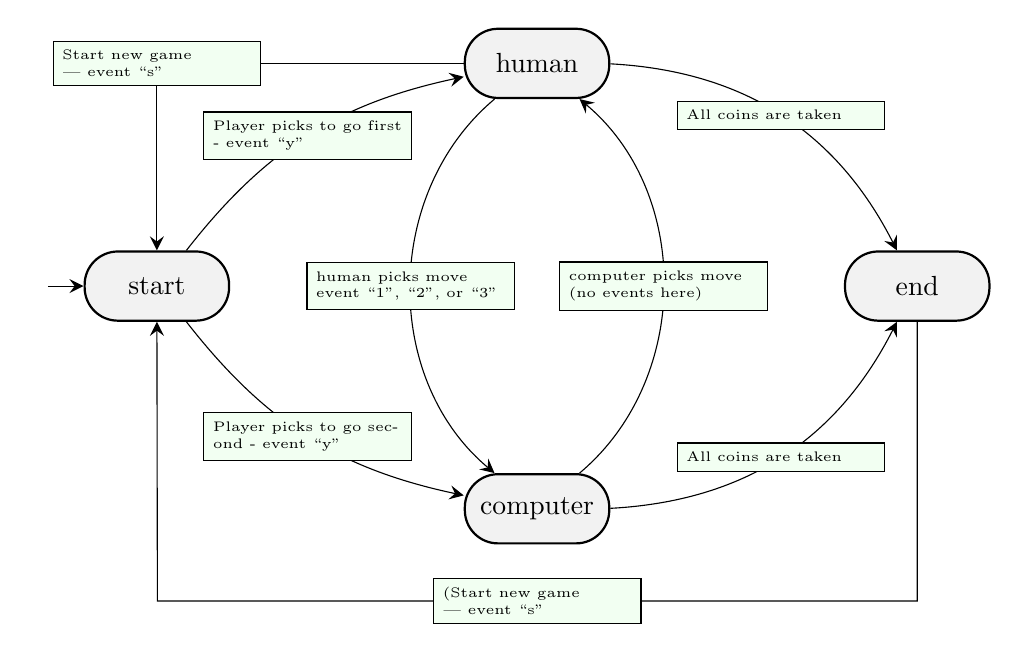
\begin{tikzpicture}

\tikzset{
        ->,  % makes the edges directed
        >=stealth, % makes the arrow heads bold
        very thick,
        draw=blue,
        node distance=4cm, % specifies the minimum distance between two nodes. Change if n
        every state/.style={black,text width=1.6cm,shape=rectangle,rounded corners=12pt,align=center,thick, fill=gray!10}, % sets the properties for each ?state? n
        initial text=$ $, % sets the text that appears on the start arrow
        }
        
        
        \node[state, initial] (start) {start};

        \node[state, above right of=start,xshift=2cm] (human) {human};
        \node[state, below right of=start,xshift=2cm] (computer) {computer};
        \node[state, below right of=human,xshift=2cm] (end) {end};

        \tikzstyle{l}=[fill=green!05,draw,font={\smaller[3]},text width=2.4cm]
        
        \draw (start) to[bend left=20] node[l]{Player picks to go first - event ``y''} (human);
        \draw (start) to[bend right=20] node[l]{Player picks to go second - event ``y''} (computer);

        \draw (human) to[bend right=50] node[l]{human picks move\\event ``1'', ``2'', or ``3''} (computer);
        \draw (computer) to[bend right=50] node[l]{computer picks move\\ (no events here)} (human);

        \draw (human) to[bend left=30] node[l]{All coins are taken} (end);
        \draw (computer) to[bend right=30] node[l]{All coins are taken} (end);

        \draw (human) -|  node[l] {Start new game\\--- event ``s''} (start);

        \draw (end) -- ++(0,-4) -- node [l] {(Start new game\\--- event ``s''}  ++(-9.65,0)  -- (start);

\end{tikzpicture}

\end{document}
